% -*- latex -*-
%%%%%%%%%%%%%%%%%%%%%%%%%%%%%%%%%%%%%%%%%%%%%%%%%%%%%%%%%%%%%%%%
%%%%%%%%%%%%%%%%%%%%%%%%%%%%%%%%%%%%%%%%%%%%%%%%%%%%%%%%%%%%%%%%
%%%%
%%%% This text file is part of the source of 
%%%% `Introduction to High-Performance Scientific Computing'
%%%% by Victor Eijkhout, copyright 2012-8
%%%%
%%%% This book is distributed under a Creative Commons Attribution 3.0
%%%% Unported (CC BY 3.0) license and made possible by funding from
%%%% The Saylor Foundation \url{http://www.saylor.org}.
%%%%
%%%% debug.tex : tutorial for debugging
%%%%
%%%%%%%%%%%%%%%%%%%%%%%%%%%%%%%%%%%%%%%%%%%%%%%%%%%%%%%%%%%%%%%%
%%%%%%%%%%%%%%%%%%%%%%%%%%%%%%%%%%%%%%%%%%%%%%%%%%%%%%%%%%%%%%%%

\index{debugging|(}

\begin{quotation}
  Debugging is like being the detective in a crime movie where you are
  also the murderer. (Filipe Fortes, 2013)
\end{quotation}

When a program misbehaves, \emph{debugging} is the process of finding
out \emph{why}.
There are various strategies of finding errors in a program.
The crudest one is debugging by print statements. If you have a
notion of where in your code the error arises, you can edit your code
to insert print statements, recompile, rerun, and see if the output
gives you any suggestions. There are several problems with this:
\begin{itemize}
\item The edit/compile/run cycle is time consuming, especially since
\item often the error will be caused by an earlier section of code,
  requiring you to edit, compile, and rerun repeatedly. Furthermore,
\item the amount of data produced by your program can be too large to
  display and inspect effectively, and
\item if your program is parallel, you probably need to print out data
  from all proccessors, making the inspection process very tedious.
\end{itemize}

\index{gdb|(}

For these reasons, the best way to debug is by the use of an
interactive \indexterm{debugger}, a program that allows you to monitor
and control the behaviour of a running program. In this section you
will familiarize yourself with
\emph{gdb}\index{GNU!gdb|see{gdb}}, which is the open source
debugger of the \indexterm{GNU} project. Other debuggers are
proprietary, and typically come with a compiler suite. Another
distinction is that gdb is a commandline debugger; there are
graphical debuggers such as \indexterm{ddd} (a~frontend to gdb) or
\indexterm{DDT} and \indexterm{TotalView} (debuggers for parallel
codes). We limit ourselves to gdb, since it incorporates the basic
concepts common to all debuggers.

In this tutorial you will debug a number of simple programs with
gdb and valgrind. The files can be found in the repository
in the directory \n{tutorials/debug_tutorial_files}.


\Level 0 {Invoking {\tt gdb}}

There are three ways of using gdb: using it to start a program,
attaching it to an already running program, or using it to inspect a
\indexterm{core dump}. We will only consider the first possibility.

Here is an exaple of how to start gdb with program that has no
arguments (Fortran users, use \n{hello.F}):
\codelisting{tutorials/gdb/c/hello.c}
\begin{verbatim}
%% cc -g -o hello hello.c
# regular invocation:
%% ./hello
hello world
# invocation from gdb:
%% gdb hello
GNU gdb 6.3.50-20050815 # ..... version info
Copyright 2004 Free Software Foundation, Inc. .... copyright info ....
(gdb) run
Starting program: /home/eijkhout/tutorials/gdb/hello 
Reading symbols for shared libraries +. done
hello world

Program exited normally.
(gdb) quit
%%
\end{verbatim}

Important note: the program was compiled with the \indexterm{debug
  flag}~\n{-g}. This causes the \indexterm{symbol table} (that is, the
translation from machine address to program variables) and other debug
information to be included in the binary. This will make your binary
larger than strictly necessary, but it will also make it slower, for
instance because the compiler will not perform certain
optimizations\footnote{Compiler optimizations are not supposed to
  change the semantics of a program, but sometimes do. This can lead
  to the nightmare scenario where a program crashes or gives incorrect
  results, but magically works correctly with compiled with debug and
  run in a debugger.}.

To illustrate the presence of the symbol table do
\begin{verbatim}
%% cc -g -o hello hello.c
%% gdb hello
GNU gdb 6.3.50-20050815 # ..... version info
(gdb) list
\end{verbatim}
and compare it with leaving out the \n{-g} flag:
\begin{verbatim}
%% cc -o hello hello.c
%% gdb hello
GNU gdb 6.3.50-20050815 # ..... version info
(gdb) list
\end{verbatim}

For a program with commandline input we give the arguments to the
\n{run} command (Fortran users use \n{say.F}):
\codelisting{tutorials/gdb/c/say.c}
\begin{verbatim}
%% cc -o say -g say.c
%% ./say 2
hello world
hello world
%% gdb say
.... the usual messages ...
(gdb) run 2
Starting program: /home/eijkhout/tutorials/gdb/c/say 2
Reading symbols for shared libraries +. done
hello world
hello world

Program exited normally.
\end{verbatim}

\Level 0 {Finding errors}

Let us now consider some programs with errors.

\Level 1 {C programs}

%\codelisting{tutorials/gdb/c/square.c}
\verbatimsnippet{gdb-square}
\begin{verbatim}
%% cc -g -o square square.c
 %% ./square
5000
Segmentation fault
\end{verbatim}
The \indexterm{segmentation fault} (other messages are possible too) 
indicates that we are accessing
memory that we are not allowed to, making the program
abort. A~debugger will quickly tell us where this happens:
\begin{verbatim}
%% gdb square
(gdb) run
50000

Program received signal EXC_BAD_ACCESS, Could not access memory.
Reason: KERN_INVALID_ADDRESS at address: 0x000000000000eb4a
0x00007fff824295ca in __svfscanf_l ()
\end{verbatim}
Apparently the error occurred in a function \n{__svfscanf_l}, which is
not one of ours, but a system function. Using the \n{backtrace}
(or~\n{bt}, also \n{where} or~\n{w}) command we
display the \indexterm{call stack}. This usually allows us to find out
where the error lies:
{\small
\begin{verbatim}
(gdb) backtrace
#0  0x00007fff824295ca in __svfscanf_l ()
#1  0x00007fff8244011b in fscanf ()
#2  0x0000000100000e89 in main (argc=1, argv=0x7fff5fbfc7c0) at square.c:7
\end{verbatim}
}
We take a close look at line~7, and see that we need to
change \n{nmax} to~\n{&nmax}.

There is still an error in our program:
{\small
\begin{verbatim}
(gdb) run
50000

Program received signal EXC_BAD_ACCESS, Could not access memory.
Reason: KERN_PROTECTION_FAILURE at address: 0x000000010000f000
0x0000000100000ebe in main (argc=2, argv=0x7fff5fbfc7a8) at square1.c:9
9           squares[i] = 1./(i*i); sum += squares[i];
\end{verbatim}
}
We investigate further:
\begin{verbatim}
(gdb) print i
$1 = 11237
(gdb) print squares[i]
Cannot access memory at address 0x10000f000
(gdb) print squares
$2 = (float *) 0x0
\end{verbatim}
and we quickly see that we forgot to allocate \n{squares}.

Memory errors can also occur if we have a legitimate array, but we access it
outside its bounds.
\verbatimsnippet{gdb-up}
\begin{verbatim}
Program received signal EXC_BAD_ACCESS, Could not access memory.
Reason: KERN_INVALID_ADDRESS at address: 0x0000000100200000
0x0000000100000f43 in main (argc=1, argv=0x7fff5fbfe2c0) at up.c:15
15          s += array[i];
(gdb) print array
$1 = (double *) 0x100104d00
(gdb) print i
$2 = 128608
\end{verbatim}

\Level 1 {Fortran programs}

Compile and run the following program:
\codelisting{tutorials/gdb/f/square.F}
It should abort with a message such as `Illegal instruction'.
Running the program in gdb quickly tells you where the problem lies:
\begin{verbatim}
(gdb) run
Starting program: tutorials/gdb//fsquare 
Reading symbols for shared libraries ++++. done

Program received signal EXC_BAD_INSTRUCTION,
Illegal instruction/operand.
0x0000000100000da3 in square () at square.F:7
7                sum = sum + squares(i)
\end{verbatim}
We take a close look at the code and see that we did not allocate
\n{squares} properly.

\Level 0 {Memory debugging with Valgrind}
\label{sec:valgrind}

Insert the following allocation of \n{squares} in your program:
\begin{verbatim}
squares = (float *) malloc( nmax*sizeof(float) );
\end{verbatim}
Compile and run your program. The output will likely be correct,
although the program is not. Can you see the problem?

\index{valgrind|(}

To find such subtle memory errors you need a different tool: a memory
debugging tool. A~popular (because open source) one is
\emph{valgrind}; a~common commercial tool is \indexterm{purify}.

\codelisting{tutorials/gdb/c/square1.c}
%
Compile this program with \n{cc -o square1 square1.c} and run it with
\n{valgrind square1} (you need to type the input value). You will lots
of output, starting with:
{\small
\begin{verbatim}
%% valgrind square1
==53695== Memcheck, a memory error detector
==53695== Copyright (C) 2002-2010, and GNU GPL'd, by Julian Seward et al.
==53695== Using Valgrind-3.6.1 and LibVEX; rerun with -h for copyright info
==53695== Command: a.out
==53695== 
10
==53695== Invalid write of size 4
==53695==    at 0x100000EB0: main (square1.c:10)
==53695==  Address 0x10027e148 is 0 bytes after a block of size 40 alloc'd
==53695==    at 0x1000101EF: malloc (vg_replace_malloc.c:236)
==53695==    by 0x100000E77: main (square1.c:8)
==53695== 
==53695== Invalid read of size 4
==53695==    at 0x100000EC1: main (square1.c:11)
==53695==  Address 0x10027e148 is 0 bytes after a block of size 40 alloc'd
==53695==    at 0x1000101EF: malloc (vg_replace_malloc.c:236)
==53695==    by 0x100000E77: main (square1.c:8)
\end{verbatim}
}
Valgrind is informative but cryptic, since it works on the bare
memory, not on variables. Thus, these error messages take some
exegesis. They state that a line 10 writes a 4-byte object immediately
after a block of 40 bytes that was allocated. In other words: the code
is writing outside the bounds of an allocated array. Do you see what
the problem in the code is?

Note that valgrind also reports at the end of the program run how much
memory is still in use, meaning not properly \n{free}d.

If you fix the array bounds and recompile and rerun the program,
valgrind still complains:
{\small
\begin{verbatim}
==53785== Conditional jump or move depends on uninitialised value(s)
==53785==    at 0x10006FC68: __dtoa (in /usr/lib/libSystem.B.dylib)
==53785==    by 0x10003199F: __vfprintf (in /usr/lib/libSystem.B.dylib)
==53785==    by 0x1000738AA: vfprintf_l (in /usr/lib/libSystem.B.dylib)
==53785==    by 0x1000A1006: printf (in /usr/lib/libSystem.B.dylib)
==53785==    by 0x100000EF3: main (in ./square2)
\end{verbatim}
}
Although no line number is given, the mention of \n{printf} gives an
indication where the problem lies.
The reference to an `uninitialized value' is again cryptic: the only
value being output is \n{sum}, and that is not uninitialized: it has
been added to several times. Do you see why valgrind calls it
uninitialized all the same?

\index{valgrind|)}

\Level 0 {Stepping through a program}

Often the error in a program is sufficiently obscure that you need to
investigate the program run in detail. Compile the following program
%
\codelisting{tutorials/gdb/c/roots.c}
%
and run it:
\begin{verbatim}
%% ./roots
sum: nan
\end{verbatim}
Start it in gdb as before:
\begin{verbatim}
%% gdb roots
GNU gdb 6.3.50-20050815 
Copyright 2004 Free Software Foundation, Inc.
....
\end{verbatim}
but before you run the program, you set a \indexterm{breakpoint}
at \n{main}.
This tells the execution to stop, or `break', in the main program.
\begin{verbatim}
(gdb) break main
Breakpoint 1 at 0x100000ea6: file root.c, line 14.
\end{verbatim}
Now the program will stop at the first executable statement in \n{main}:
\begin{verbatim}
(gdb) run
Starting program: tutorials/gdb/c/roots
Reading symbols for shared libraries +. done

Breakpoint 1, main () at roots.c:14
14        float x=0;
\end{verbatim}

If execution is stopped at a breakpoint, you can do various things,
such as issuing the \n{step} command:
\begin{verbatim}
Breakpoint 1, main () at roots.c:14
14        float x=0;
(gdb) step
15        for (i=100; i>-100; i--)
(gdb) 
16          x += root(i);
(gdb) 
\end{verbatim}
(if you just hit return, the previously issued command is
repeated). Do a number of \n{step}s in a row by hitting return. What
do you notice about the function and the loop?

Switch from doing \n{step} to doing \n{next}. Now what do you notice
about the loop and the function? 

Set another breakpoint: \n{break 17} and do \n{cont}. What happens?

Rerun the program after you set a breakpoint on the line with the
\n{sqrt} call. When the execution stops there do \n{where} and
\n{list}.

\Level 0 {Inspecting values}

Run the previous program again in gdb: set a breakpoint at the line
that does the \n{sqrt} call before you actually call \n{run}. When the
program gets to line~8 you can do \n{print n}. Do \n{cont}. Where does
the program stop?

If you want to repair a variable, you can do \n{set var=value}. Change
the variable \n{n} and confirm that the square root of the new value
is computed. Which commands do you do?

\Level 0 {Breakpoints}
\index{breakpoint|(textbf}

If a problem occurs in a loop, it can be tedious keep typing \n{cont}
and inspecting the variable with \n{print}. Instead you can add a
condition to an existing breakpoint. First of all, you can make the breakpoint
subject to a condition: with
\begin{verbatim}
condition 1 if (n<0)
\end{verbatim}
breakpoint~1 will only obeyed if \texttt{n<0} is true.

You can also have a breakpoint that is only activated by some condition.
The statement
\begin{verbatim}
break 8 if (n<0)
\end{verbatim}
means that breakpoint~8 becomes (unconditionally) active after
the condition \texttt{n<0} is encountered.

Another possibility is to use \n{ignore 1 50}, which will not stop at
breakpoint 1 the next 50 times.

Remove the existing breakpoint, redefine it with the condition \n{n<0}
and rerun your program. When the program breaks, find for what value
of the loop variable it happened. What is the sequence of commands you use?

You can set a breakpoint in various ways:
\begin{itemize}
\item \n{break foo.c} to stop when code in a certain file is reached;
\item \n{break 123} to stop at a certain line in the current file;
\item \n{break foo} to stop at subprogram \n{foo}
\item or various combinations, such as \n{break foo.c:123}.
\item Finally, 
\end{itemize}

\begin{itemize}
\item If you set many breakpoints, you can find out what they are with
  \n{info breakpoints}. 
\item You can remove breakpoints with \n{delete n} where \n{n} is the
  number of the breakpoint.
\item If you restart your program with \n{run} without leaving gdb,
  the breakpoints stay in effect.
\item If you leave gdb, the breakpoints are cleared but you can save
  them: \n{save breakpoints <file>}. Use \n{source <file>} to read
  them in on the next gdb run.
\end{itemize}

Finally, you can execute commands at a breakpoint:
\begin{verbatim}
break 45
command
print x
cont
end
\end{verbatim}
This states that at line 45 variable~\n{x} is to be printed, and execution
should immediately continue.

If you want to run repeated gdb sessions on the same program,
you may want to save an reload breakpoints. This can be done with
\begin{verbatim}
save-breakpoint filename
source filename
\end{verbatim}

\index{breakpoint|)}
\index{gdb|)}

\Level 0 {Parallel debugging}
\index{debugging!in parallel|(}

\begin{figure}[ht]
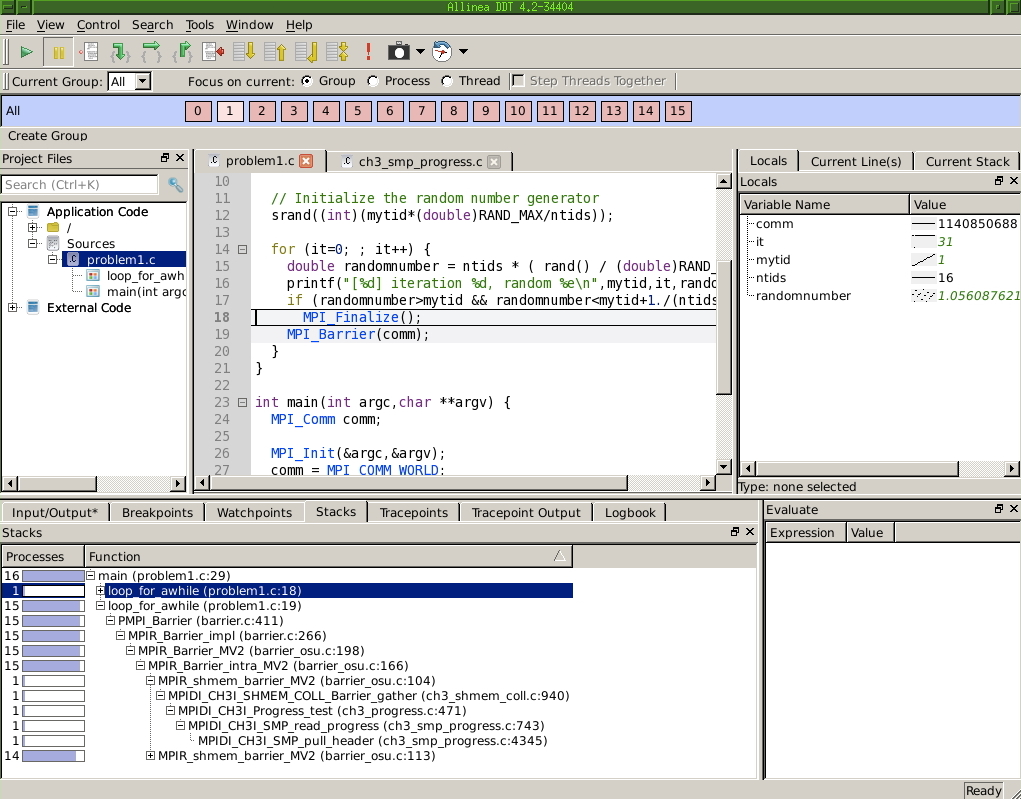
\includegraphics[scale=.4]{ddt2}
\caption{Display of 16 processes in the DDT debugger}
\label{fig:ddt2}
\end{figure}

Debugging in parallel is harder than sequentially, because you will run
errors that are only due to interaction of processes such as \indexterm{deadlock};
see section~\ref{sec:nonblocking}.

As an example, consider this segment of MPI code:
\begin{verbatim}
MPI_Init(0,0);
// set comm, ntids, mytid
for (int it=0; ; it++) {
  double randomnumber = ntids * ( rand() / (double)RAND_MAX );
  printf("[%d] iteration %d, random %e\n",mytid,it,randomnumber);
  if (randomnumber>mytid && randomnumber<mytid+1./(ntids+1))  
    MPI_Finalize();
}
MPI_Finalize();
\end{verbatim}
Each process computes random numbers until a certain condition is satisfied, then exits.
However, consider introducing a barrier (or something that acts like it, such as a reduction):
\begin{verbatim}
for (int it=0; ; it++) {
  double randomnumber = ntids * ( rand() / (double)RAND_MAX );
  printf("[%d] iteration %d, random %e\n",mytid,it,randomnumber);
  if (randomnumber>mytid && randomnumber<mytid+1./(ntids+1))  
    MPI_Finalize();
  MPI_Barrier(comm);
}
MPI_Finalize();
\end{verbatim}
Now the execution will hang, and this is not due to any particular process:
each process has a code path from init to finalize that does not develop
any memory errors or other runtime errors.
However as soon as one process reaches the finalize call in the conditional
it will stop, and all other processes will be waiting at the barrier.

Figure~\ref{fig:ddt2} shows the main display of the Allinea \indextermdef{DDT}
debugger (\url{http://www.allinea.com/products/ddt}) at the point where this code stops.
Above the source panel you see that there are 16 processes, and that the status is given
for process~1.
In the bottom display you see that out of 16 processes 15~are calling \n{MPI_Barrier} on line~19,
while one is at line~18. In the right display you see a listing of the local variables:
the value specific to process~1. A~rudimentary graph displays the values over the processors:
the value of \n{ntids} is constant, that of \n{mytid} is linearly increasing, and \n{it}
is constant except for one process.

\begin{exercise}
  Make and run \n{ring_1a}. The program does not terminate and does not crash.
  In the debugger you can interrupt the execution, and see that all processes
  are executing a receive statement. This is probably a case of deadlock.
  Diagnose and fix the error.
\end{exercise}

\begin{exercise}
  The author of \n{ring_1c} was very confused about how MPI works. Run the program.
  While it terminates without a problem, the output is wrong. Set a breakpoint
  at the send and receive statements to figure out what is happening.
\end{exercise}


\index{debugging!in parallel|)}

\Level 0 {Further reading}

A good tutorial: \url{http://www.dirac.org/linux/gdb/}.

Reference manual: \url{http://www.ofb.net/gnu/gdb/gdb_toc.html}.

\index{debugging|)}
